\documentclass[11pt,paper=a4,final]{scrartcl}
\usepackage[utf8]{inputenc}
\usepackage{geometry}           %allows us to specify the 'seitenrand'
\usepackage{graphicx}           %package used to include graphics
\usepackage{hyperref}           %used to make klickable links
\usepackage{listings}
\usepackage{tabularx}
\usepackage{pdflscape}
\usepackage[figuresright]{rotating}
\usepackage{nameref}
\usepackage{longtable}
\usepackage{enumitem}
\usepackage{footnote} % Make the document German
\usepackage{ngerman}
% allow rowspan
\usepackage{multirow}

\hypersetup{
    colorlinks,
    citecolor=black,
    filecolor=black,
    linkcolor=black,
    urlcolor=black
}

\usepackage{fancyhdr}
\pagestyle{fancy}
% \setlength{\parskip}{0pt}
% \setlength{\baselineskip}{0pt}
%\parindent 0pt 
%\parskip 11pt
%\parsep 0pt 
%\itemsep 0pt 
%\topsep 0pt 

\geometry{a4paper, top=20mm, right=20mm, bottom=20mm, left=20mm}

%defining header and footer
\fancyhf{}      %delete default values
\setlength{\headwidth}{\textwidth}      %header and footer width equal the text width
%\fancyhead[LE,LO]{\includegraphics[scale=0.6]{header.png}}
\fancyhead[LE,LO]{Roland Peka Rytz, Niklaus Manuel Hofer}
\fancyhead[RE,RO]{Chromatographie}
\fancyfoot[CE,CO]{Speicherdatum: \today{}}
\fancyfoot[RE,RO]{\thepage}

%New page for every section
%\let\stdsection\section
%\renewcommand\section{\newpage\stdsection}

\title{Chromatographie}
\author{Roland Peka Rytz, Niklaus Manuel Hofer}
\date{\today{}}

\begin{document}
\maketitle

\section{Messwerte, Beobachtungen}
\subsection{Messwerte}
Genauigkeit der Chromatographie-Platten: unbekannt\\
Genauigkeit der Messung (siehe unten): \( \pm 0.3cm\) \\
Ungenauigkeit beim Vermessen der L\"osungsmittel-Front: vernachl\"assigbar \\
Die Temepratur im Arbeitszimmer betrug: \(20^\circ C \pm 3^\circ C\)
\subsection{Stifte und gegebene Mischung}
\begin{savenotes} %Handles footnotes within tables
  \begin{table}[ht!]
    \centering
    \begin{tabular}{|l|l|l|l|}
      \hline
    \bf Farbe Nr.	& \bf Teilfarbe	& \bf \(R_{Lsm}\)		& \bf Distanz (\(R_x\))	\\ \hline
      1 (Hellblau)	& Hellblau	& \multirow{6}{*}{6.1 cm }	& 4.0 cm \(\pm 3 mm \)	\\ \cline{1-2} \cline{4-4}
      2 (Dunkelgr\"un)	& Dunkelgr\"un	&				& 5.8 cm \(\pm 3 mm \)	\\ \cline{1-2} \cline{4-4}
      \multirow{2}{*}{3 (rot) }
			& Pink		&				& 4.6 cm \(\pm 3 mm \)	\\ 
			& Orange	&				& 6.1 cm 		\\ \cline{1-2} \cline{4-4}
      \multirow{2}{*}{4 (Hellgr\"un) }
 			& Hellblau	&				& 3.3 cm \(\pm 3 mm \)	\\
			& Gelb		&				& 6.1 cm		\\ \hline
      5 (gelb)		& Orange	& \multirow{10}{*}{6.1 cm }	& 6.1 cm		\\ \cline{1-2} \cline{4-4}
      \multirow{4}{*}{6 (Braun)}
			& Violett	&				& 0.7 cm \(\pm 3 mm \)	\\
			& Hellblau	&				& 2.7 cm \(\pm 3 mm \)	\\
      			& pink		&				& 3.9 cm \(\pm 3 mm \)	\\
      			& Orange	&				& 6.1 cm 		\\ \cline{1-2} \cline{4-4}
      \multirow{2}{*}{7 (Schwarz}
      			& Gelb		&				& 4.0 cm \(\pm 6 mm \)	\\
      			& Schwarz	&				& 6.1 cm		\\ \cline{1-2} \cline{4-4}
      \multirow{3}{*}{8 (Rot)}
      			& Dunkelpink	& 				& 1.6 cm \(\pm 3 mm \)	\\ 
      			& Hellpink	&				& 4.7 cm \(\pm 3 mm \)	\\
      			& Orange	&				& 6.1 cm		\\ \hline
      9 (t\"urkis)	& T\"urkis	& \multirow{6}{*}{6.0 cm }	& 3.5 cm \(\pm 3 mm \)	\\ \cline{1-2} \cline{4-4}
       10 (orange)	& Orange	& 				& 6.0 cm		\\ \cline{1-2} \cline{4-4}
      \multirow{3}{*}{11 (Violett)}
      			& Dunkelpink	&				& 1.9 cm \(\pm 3 mm \)	\\
      			& Hellpink	&				& 2.3 cm \(\pm 3 mm \)	\\
      			& Blau		&				& 6.0 cm		\\ \cline{1-2} \cline{4-4}
      12 (pink)		& Pink		&				& 0.3 cm \(\pm 1 mm \)	\\ \hline
      \multirow{4}{*}{Mischung 4}
      			& Violett	& \multirow{4}{*}{6.0 cm }	& 0.6 cm \(\pm 2 mm \)	\\
      			& Dunkelpink	&				& 1.2 cm \(\pm 3 mm \)	\\
			& Blau		& 				& 2.7 cm \(\pm 3 mm \)	\\
      			& Hellpink	& 				& 3.6 cm \(\pm 3 mm \)	\\ \hline
      	
    \end{tabular}
    \caption{Messergebnisse}
  \end{table}
\end{savenotes}

\subsection{Eigene Mischungen}
\begin{savenotes}
  \begin{table}[ht!]
    \centering
    \begin{tabular}{|l|l|}
      \hline
      \bf Name & \bf Verwendete Stifte	\\ \hline
      A & 5 + 6 			\\ \hline
      B & 10 + 5			\\ \hline
      C & 10 + 6 			\\ \hline
      D & 6 + 5 + 10			\\ \hline
      E & 6 + 3				\\ \hline
      F & (unbekannt)			\\ \hline
      G & 6 + 11			\\ \hline
      H & 6 + 8				\\ \hline
    \end{tabular}
    \caption{Eigene Mischungen}
  \end{table}
\end{savenotes}

\begin{savenotes}
  \begin{table}[ht!]
    \centering
    \begin{tabular}{|l|l|l|l|}
      \hline
      \bf Mischung	& \bf Teilfarbe	& \bf \(R_{Lsm}\)		& \bf Distanz (\(R_x\))	\\ \hline
      \multirow{4}{*}{A}
			& Violett	& \multirow{13}{*}{4.8 cm }	& 0.9 cm \(\pm 3 mm \)	\\
      			& Blau		& 				& 2.6 cm \(\pm 3 mm \)	\\
      			& Pink		&				& 3.1 cm \(\pm 3 mm \)	\\
      			& Orange	&				& 4.8 cm 		\\ \cline{1-2} \cline{4-4}
       B		& Orange	&				& 4.8 cm		\\ \cline{1-2} \cline{4-4}
      \multirow{4}{*}{C}
			& Violett	& 				& 0.9 cm \(\pm 3 mm \)	\\
      			& Blau		& 				& 2.6 cm \(\pm 3 mm \)	\\
      			& Pink		&				& 3.1 cm \(\pm 3 mm \)	\\
      			& Orange	&				& 4.8 cm 		\\ \cline{1-2} \cline{4-4}
      \multirow{4}{*}{D}
			& Violett	&				& 0.9 cm \(\pm 3 mm \)	\\
      			& Blau		& 				& 2.6 cm \(\pm 3 mm \)	\\
      			& Pink		&				& 3.1 cm \(\pm 3 mm \)	\\
      			& Orange	&				& 4.8 cm 		\\ \hline
      \multirow{4}{*}{E}
			& Violett	& \multirow{18}{*}{4.6 cm }	& 1.2 cm \(\pm 3 mm \)	\\
      			& Blau		& 				& 2.7 cm \(\pm 3 mm \)	\\
      			& Pink		&				& 3.3 cm \(\pm 3 mm \)	\\
			      & orange	&				& 4.6 cm 		\\ \cline{1-2} \cline{4-4}
      \multirow{4}{*}{F}
			& Violett	&				& 1.2 cm \(\pm 3 mm \)	\\
      			& Blau		& 				& 2.7 cm \(\pm 3 mm \)	\\
      			& Pink		&				& 3.5 cm \(\pm 3 mm \)	\\
			& Orange	&				& 4.6 cm 		\\ \cline{1-2} \cline{4-4}
      \multirow{5}{*}{G}
			& Violett	&				& 1.3 cm \(\pm 3 mm \)	\\
      			& Dunkelpink 	&				& 1.7 cm \(\pm 3 mm \)	\\
			& Blau		&				& 2.6 cm \(\pm 3 mm \)	\\
      			& Hellpink	& 				& 3.1 cm \(\pm 3 mm \)	\\
      			& Orange	&				& 4.6 cm		\\ \cline{1-2} \cline{4-4}
      \multirow{5}{*}{F}
			& Violett	&				& 1.2 cm \(\pm 3 mm \)	\\
      			& Dunkelpink 	&				& 1.5 cm \(\pm 3 mm \)	\\
      			& Blau		& 				& 2.7 cm \(\pm 3 mm \)	\\
      			& Pink		&				& 3.5 cm \(\pm 3 mm \)	\\
			& Orange	&				& 4.6 cm 		\\ \hline

    \end{tabular}
    \caption{Messergebnisse bei den Mischungen}
  \end{table}
\end{savenotes}

\section{Berechnungen, Resultate}
Die Formel zur Berechnung von \(R_f\) lautet wie folgt: \(R_f = \frac{R_x}{R_{Lsm}} \) \\
Wobei gilt:\\
\(R_x\): Laufstrecke der Substanz\\
\(R_{Lsm}\): Laufstrecke des L\"osungsmittels

\subsection{Stifte und gegebene Mischung}
\begin{savenotes} %Handles footnotes within tables
  \begin{table}[ht!]
    \centering
    \begin{tabular}{|l|l|l|l|l|}
      \hline
    \bf Farbe Nr.	& \bf Teilfarbe	& \bf \(R_{Lsm}\)		& \bf Distanz (\(R_x\))	& \bf \(R_f\)		\\ \hline
      1 (Hellblau)	& Hellblau	& \multirow{6}{*}{6.1 cm }	& 4.0 cm \(\pm 3 mm \)	& 0.607 - 0.705		\\ \cline{1-2} \cline{4-5}
      2 (Dunkelgr\"un)	& Dunkelgr\"un	&				& 5.8 cm \(\pm 3 mm \)	& 0.902 - 1.000		\\ \cline{1-2} \cline{4-5}
      \multirow{2}{*}{3 (rot) }
			& Pink		&				& 4.6 cm \(\pm 3 mm \)	& 0.705 - 0.803		\\ 
			& Orange	&				& 6.1 cm 		& 1.00 (nicht definiert)\\ \cline{1-2} \cline{4-5}
      \multirow{2}{*}{4 (Hellgr\"un) }
 			& Hellblau	&				& 3.3 cm \(\pm 3 mm \)	& 0.500 - 0.600		\\
			& Gelb		&				& 6.1 cm		& 1.00 (nicht definiert)\\ \hline
      5 (Gelb)		& Orange	& \multirow{10}{*}{6.1 cm }	& 6.1 cm		& 1.00 (nicht definiert)\\ \cline{1-2} \cline{4-5}
      \multirow{4}{*}{6 (Braun)}
			& Violett	&				& 0.7 cm \(\pm 3 mm \)	& 0.066 - 0.164		\\
			& Hellblau	&				& 2.7 cm \(\pm 3 mm \)	& 0.393 - 0.492		\\
      			& Pink		&				& 3.9 cm \(\pm 3 mm \)	& 0.590 - 0.689		\\
      			& Orange	&				& 6.1 cm 		& 1.00 (nicht definiert)\\ \cline{1-2} \cline{4-5}
      \multirow{2}{*}{7 (Schwarz}
      			& Gelb		&				& 4.0 cm \(\pm 6 mm \)	& 0.557 - 0.754		\\
      			& Schwarz	&				& 6.1 cm		& 1.00 (nicht definiert)\\ \cline{1-2} \cline{4-5}
      \multirow{3}{*}{8 (Rot)}
      			& Dunkelpink	& 				& 1.6 cm \(\pm 3 mm \)	& 0.213 - 0.311		\\ 
      			& Hellpink	&				& 4.7 cm \(\pm 3 mm \)	& 0.721 - 0.820		\\
      			& Orange	&				& 6.1 cm		& 1.00 (nicht definiert)\\ \hline
      9 (T\"urkis)	& T\"urkis	& \multirow{6}{*}{6.0 cm }	& 3.5 cm \(\pm 3 mm \)	& 0.533 - 0.633		\\ \cline{1-2} \cline{4-5}
       10 (Orange)	& Orange	& 				& 6.0 cm		& 1.00 (nicht definiert)\\ \cline{1-2} \cline{4-5}
      \multirow{3}{*}{11 (Violett)}
      			& Dunkelpink	&				& 1.9 cm \(\pm 3 mm \)	& 0.266 - 0.366		\\
      			& Hellpink	&				& 2.3 cm \(\pm 3 mm \)	& 0.333 - 0.433		\\
      			& Blau		&				& 6.0 cm		& 1.00 (nicht definiert \\ \cline{1-2} \cline{4-5}
      12 (pink)		& Pink		&				& 0.3 cm \(\pm 1 mm \)	& 0.033 - 0.066		\\ \hline
      \multirow{4}{*}{Mischung 4}
      			& Violett	& \multirow{4}{*}{6.0 cm }	& 0.6 cm \(\pm 2 mm \)	& 0.066 - 0.133		\\
      			& Dunkelpink	&				& 1.2 cm \(\pm 3 mm \)	& 0.150 - 0.250		\\
			& Blau		& 				& 2.7 cm \(\pm 3 mm \)	& 0.400 - 0.500		\\
      			& Hellpink	& 				& 3.6 cm \(\pm 3 mm \)	& 0.550 - 0.650		\\ \hline
      	
    \end{tabular}
    \caption{Berechnung der Rf-Werte der Farben}
    \end{table}
\end{savenotes}

\newpage
\subsection{Eigene Mischungen}
\begin{savenotes}
  \begin{table}[ht!]
    \centering
    \begin{tabular}{|l|l|l|l|l|}
      \hline
      \bf Mischung	& \bf Teilfarbe	& \bf \(R_{Lsm}\)		& \bf Distanz (\(R_x\))	& \(R_f\)		\\ \hline
      \multirow{4}{*}{A}
			& Violett	& \multirow{13}{*}{4.8 cm }	& 0.9 cm \(\pm 3 mm \)	& 0.125 - 0.250		\\
      			& Blau		& 				& 2.6 cm \(\pm 3 mm \)	& 0.479 - 0.604		\\
      			& Pink		&				& 3.1 cm \(\pm 3 mm \)	& 0.583 - 0.708		\\
      			& Orange	&				& 4.8 cm 		& 1.00 (nicht definiert)\\ \cline{1-2} \cline{4-5}
       B		& Orange	&				& 4.8 cm		& 1.00 (nicht definiert)\\ \cline{1-2} \cline{4-5}
      \multirow{4}{*}{C}
			& Violett	& 				& 0.9 cm \(\pm 3 mm \)	& 0.125 - 0.250		\\
      			& Blau		& 				& 2.6 cm \(\pm 3 mm \)	& 0.479 - 0.604		\\
      			& Pink		&				& 3.1 cm \(\pm 3 mm \)	& 0.583 - 0.708		\\
      			& Orange	&				& 4.8 cm 		& 1.00 (nicht definiert)\\ \cline{1-2} \cline{4-5}
      \multirow{4}{*}{D}
			& Violett	&				& 0.9 cm \(\pm 3 mm \)	& 0.125 - 0.250		\\
      			& Blau		& 				& 2.6 cm \(\pm 3 mm \)	& 0.479 - 0.604		\\
      			& Pink		&				& 3.1 cm \(\pm 3 mm \)	& 0.583 - 0.708		\\
      			& Orange	&				& 4.8 cm 		& 1.00 (nicht definiert)\\ \hline
      \multirow{4}{*}{E}
			& Violett	& \multirow{18}{*}{4.6 cm }	& 1.2 cm \(\pm 3 mm \)	& 0.196 - 0.326		\\
      			& Blau		& 				& 2.7 cm \(\pm 3 mm \)	& 0.522 - 0.652		\\
      			& Pink		&				& 3.3 cm \(\pm 3 mm \)	& 0.652 - 0.782		\\
			& Orange	&				& 4.6 cm 		& 1.00 (nicht definiert)\\ \cline{1-2} \cline{4-5}
      \multirow{4}{*}{F}
			& Violett	&				& 1.2 cm \(\pm 3 mm \)	& 0.196 - 0.326		\\
      			& Blau		& 				& 2.7 cm \(\pm 3 mm \)	& 0.522 - 0.652		\\
      			& Pink		&				& 3.5 cm \(\pm 3 mm \)	& 0.696 - 0.826		\\
			& Orange	&				& 4.6 cm 		& 1.00 (nicht definiert)\\ \cline{1-2} \cline{4-5}
      \multirow{5}{*}{G}
			& Violett	&				& 1.3 cm \(\pm 3 mm \)	& 0.217 - 0.348		\\
      			& Dunkelpink 	&				& 1.7 cm \(\pm 3 mm \)	& 0.304 - 0.435		\\
			& Blau		&				& 2.6 cm \(\pm 3 mm \)	& 0.500 - 0.630		\\
      			& Hellpink	& 				& 3.1 cm \(\pm 3 mm \)	& 0.609 - 0.739		\\
      			& Orange	&				& 4.6 cm		& 1.00 (nicht definiert \\ \cline{1-2} \cline{4-5}
      \multirow{5}{*}{F}
			& Violett	&				& 1.2 cm \(\pm 3 mm \)	& 0.196 - 0.326		\\
      			& Dunkelpink 	&				& 1.5 cm \(\pm 3 mm \)	& 0.261 - 0.391		\\
      			& Blau		& 				& 2.7 cm \(\pm 3 mm \)	& 0.522 - 0.652		\\
      			& Pink		&				& 3.5 cm \(\pm 3 mm \)	& 0.696 - 0.826		\\
			& Orange	&				& 4.6 cm 		& 1.00 (nicht definiert)\\ \hline

    \end{tabular}
    \caption{Berechung der Rf-Werte der Mischungen}
  \end{table}
\end{savenotes}

\section{Fehlerabsch\"atzung}
\begin{itemize}
  \item Die Genauigkeit der Chromatographie-Platten ist leider unbekannt.
  \item Die Messung der \( R_X \) Werte ist aber ohnehin nicht besonders genau. Auch, da nicht genau klar ist wo diese gemessen werden. Einige Farbklekse laufen nach oben langsam aus.
  \item Manche Farben sind mit dem L\"osungsmittel bis ganz nach oben zu \(R_{Lsm}\) gestiegen. Dadurch ist \(R_x = R_{Lxm} \) und der Wert \(R_f = 1.000\). Es ist aber zu vermuten, dass keine Substanz wirklich ein \(R_f\) von 1.0 hat. Um das genauer bestimmen zu k\"onnen, w\"aren l\"angere Chromatographie-Platten notwendig.
\end{itemize}
Aufgrund der oben genannten Punkte, sind die Messergebnisse nicht exakt. Besonders das Auslaufen der Farben erschwert das Bestimmen der Werte. Die Toleranzen sind oben in den Berechnungen bereits enthalten und den Tabellen zu entnehmen.

\section{Auswertung, Interpretation}
\subsection{Interpretation der \(R_f\) Werte}
Die Auswertung der Stifte zeigt, dass auch manche f\"ur das blosse Auge einheitlich erscheindenden Farben in wirklichkeit aus verschiedenen Farben zusammengesetzt sind. Es handelt sich dabei also um L\"osungen. 
\subsection{Zusammensetzung der L\"osung 4}
Die Zusammensetzung der L\"osung 4 herauszufinden erwies sich als schwierig. Es war gleich von Beginn wegs klar, dass die Farbe nummer 6 (Braun) darin enthalten sein muss. Die Zusammensetzung von Braun erf\"ullt nahezu alle Merkmale. Es enth\"alt den Violetten Anfang, die blaue 'Spitze' und ein verwaschenes Pink. Allerdings hat die L\"osung 4 noch ein st\"arkeres Pink gleich oberhalb von Violett und eine nicht genau definierbare Farbe, die bis ganz nach oben mit dem L\"osungsmittel mitl\"auft. Keines dieser Merkmale wird von Braun erf\"ullt und muss deshalb von anderen Farben herr\"uhren.

In den Versuchen A bis H haben wir jeweils Braun mit verschiedenen anderen Farben gemischt. Der Versuch B ist dabei irrelevant, da er kein Braun enth\"alt. Die Ergebnisse von A bis D sind insofern gelungen, dass sie alle eine Farbe haben, die bis zu \(R_{Lsm}\) mitgelaufen ist. Allerdings fehlt in allen drei F\"allen das starke Pink direkt oberhalb vom Violett.

Die Ergebnisse E bis H kommen der Vorgabe n\"aher. Besonders das Ergebnis von G \"uberzeugt. Die Farbe die ganz mit dem L\"osungsmittel mitgelaufen ist, ist dunkel wie bei L\"osung 4 und nicht bloss Gelb wie bei den anderen Versuchen. Ausserdem ist ein festes Pink enthalten. leider sind das Pink und Violett zusehr miteinander verlaufen. Uns hat die Zeit gefehlt um zu ermitteln ob das ein Ergebnis unexakter Arbeit ist.

Auf Grund unserer Versuche und den Ergebnissen sind wir zu dem Schluss gekommen, dass L\"osung 4 aus den gleichen Stoffen wie die Farben 6 und 11 zusammengesetzt ist.

\section{anhang}
\begin{figure}[h!]
  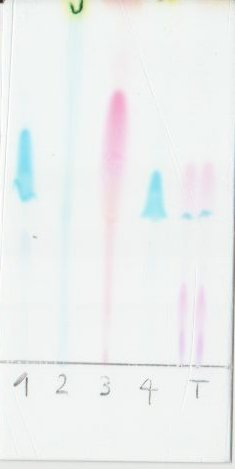
\includegraphics{1-4}
  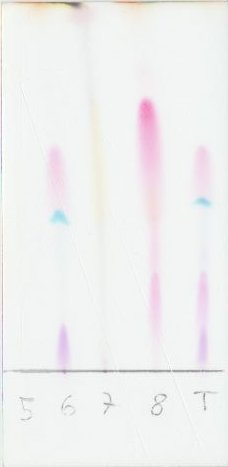
\includegraphics{5-8}
  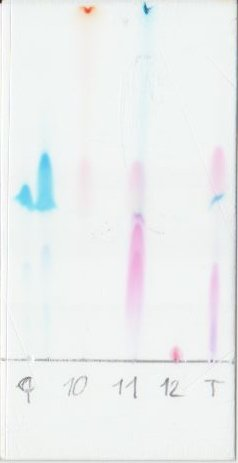
\includegraphics{9-12}
  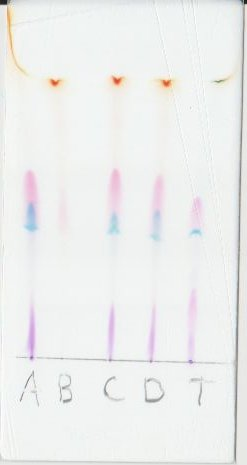
\includegraphics{a-d}
  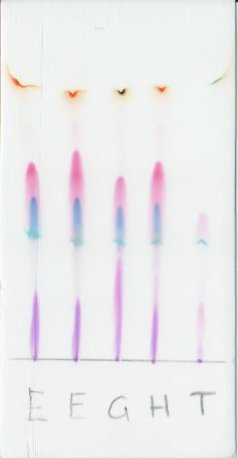
\includegraphics{e-h}
  \caption{Stifte 1 bis 4}
  \caption{Stifte 5 bis 8}
  \caption{Stifte 9 bis 12}
  \caption{Mischungen A bis D}
  \caption{Mischungen E bis H}
\end{figure}
\end{document}
